% !TeX spellcheck = en_US
\chapter{Introduction}

\section{Motivation}

\section{The IceCube Neutrino Observatory}

Since January 2011, the IceCube Neutrino Observatory at the South Pole is measuring neutrinos emanating from various sources. For this purpose a detector instrumented with digital optical modules (\enquote{DOMs}) is installed deep in the antarctic ice. 5160 of these optical sensors are arranged on 86 strings at a height between \SI{1450}{\meter} and \SI{2450}{\meter} below the surface. The central region of this In-Ice Array which has a higher density of DOMs is called \enquote{DeepCore}.

\begin{figure}[h]
	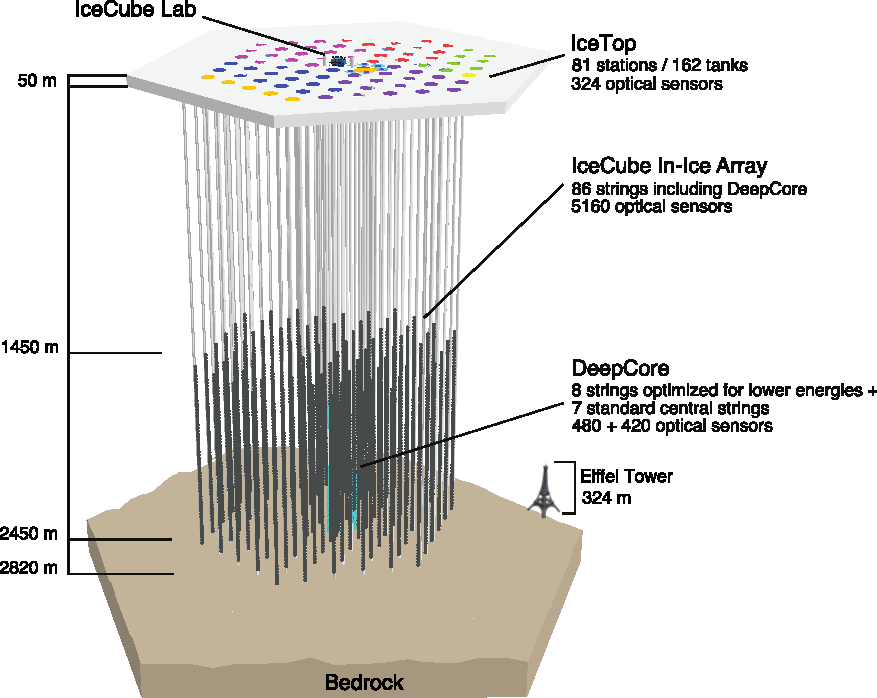
\includegraphics[width=\textwidth]{IceCubeDetector.pdf}
	\caption[Schematic view of IceCube]{\textbf{Schematic view of the IceCube Neutrino Observatory. \cite{icecube:instrumentation}} The in-ice array with the denser sub-array DeepCore as well as the surface array IceTop is sketched. Different station colors represent different deployment stages.}
\end{figure}

Neutrinos are very interesting elementary particles because of their weak interaction cross section and their electrical neutrality. This fact makes it possible for neutrinos to let them point back to their sources which is exploited in the search for astrophysical processes like active galactic nuclei, supernovae, or gamma-ray bursts. Since they are able to reach us without scattering processes, neutrinos can even give information about sources at cosmological distances. Simultaneously, the weak interaction potential is what neutrino detection makes challenging. Therefore, a detector with a large scale active volume is needed. In the case of IceCube, this is \SI{1}{\cubic\kilo\meter} of ice.

At the surface on top of the in-ice detector the cosmic ray air shower array IceTop is installed to detect Cherenkov radiation (see \ref{sec:cherenkov}). IceTop consists of 81 stations approximately arranged in the same grid as the in-ice strings. Each station has two tanks filled up with ice and two standard IceCube DOMs. This arrangement makes it possible for IceTop to detect primary cosmic rays (see \ref{sec:cosmicrays}) in the energy range of \si{\peta\electronvolt} to \si{\exa\electronvolt}. \cite{icecube:instrumentation}

\section{Air Showers and Cosmic Rays}\label{sec:cosmicrays}

\section{Atmospheric Cherenkov Light}\label{sec:cherenkov}

\section{Imaging Air Cherenkov Telescopes}

\subsection{Imaging Technique}

\subsection{Photon Detection}

\subsection{IceAct}